% Intended LaTeX compiler: pdflatex
\documentclass{scrartcl}
    \usepackage{amsmath, amssymb, bm}
		\usepackage[utf8]{inputenc}
		\usepackage[dvipdfmx]{graphicx}
		\usepackage[dvipdfmx]{color}
		\usepackage[backend=biber,bibencoding=utf8]{biblatex}
		\usepackage{url}
		\usepackage{indentfirst}
		\usepackage[normalem]{ulem}
		\usepackage{longtable}
		\usepackage{minted}
		\usepackage{fancyvrb}
    \usepackage[dvipdfmx,colorlinks=false,pdfborder={0 0 0}]{hyperref}
    \usepackage{pxjahyper}
    \usepackage{caption}

		\bibliography{reference}
\author{情報科学類3年知能情報メディア主専攻 江畑 拓哉(201611350)}
\date{}
\title{夏季進捗レポート}
\begin{document}

\maketitle
\section{概要}
\label{sec:org8318126}
\begin{enumerate}
\item deeplearning4j の理解\\
\item LSTM 式 qnaシステムの作成とその評価\\
\item データセットの作成\\
\item CopyNet, HRED の理解\\
\item seq2seq attention の理解\\
\item word2vec の理解と実装\\
\item doc2vec の利用方針\\
\item 文体変換について\\
\item 全体的なシステムの想定図\\
\end{enumerate}
\section{deeplearning4j の理解}
\label{sec:orgebe9aa7}
 Javaで書ける機械学習フレームワーク \cite{deeplearning4j} 。Tensorflow が速度と記法、記述量として不満があったのでこちらに移行した。(5分の1程度の記述量になる。またオブジェクト指向中心のためコードの再利用が楽。)\\
  また同時に比較として PyTorch (ドキュメント次第ではTensorflow) の実行結果を用いていくつもりである。(自然言語処理などではこちらの方が記述しやすい。)\\
\section{LSTM 式 qnaシステムの作成とその評価}
\label{sec:orgbd72a56}
 このシステムに注目したのは ユーモアを理解できるチャットボットについての論文 \cite{humaristbot} を読んだため、そして deeplearning4j を使った自然言語処理の例として CNN 式の qna システムがあったためです。\\
 前者では、ユーモアを理解しそれにより感情パラメータを変化させるという実験を行っています。そしてこのシステムではユーモアの理解のために AIML というマークアップ言語を用いて文章の完全ないし一部の一致検索をしている。そして文章の極性(negative or positive)を判定し、それに基づいた反応(文字、アバターの表情)をさせている。\\
 後者では以下に説明する qna タスクを VAE (Variational AutoEncoder) を用いて解決しようとしている。しかし同様のコードを作成し実行した所、芳しい結果を得られなかった \ref{fig:org25df6f9} 。そのため、Seq2Seqの考え方を利用して Seq2Label という手法を提案し \ref{fig:org3d3094e} 実験 \footnote{\url{https://github.com/MokkeMeguru/self\_introduction}\\} 、その比較を行った。\\
 結果としてかなりの精度を得ることが出来た。\\

\begin{figure}[htbp]
\centering
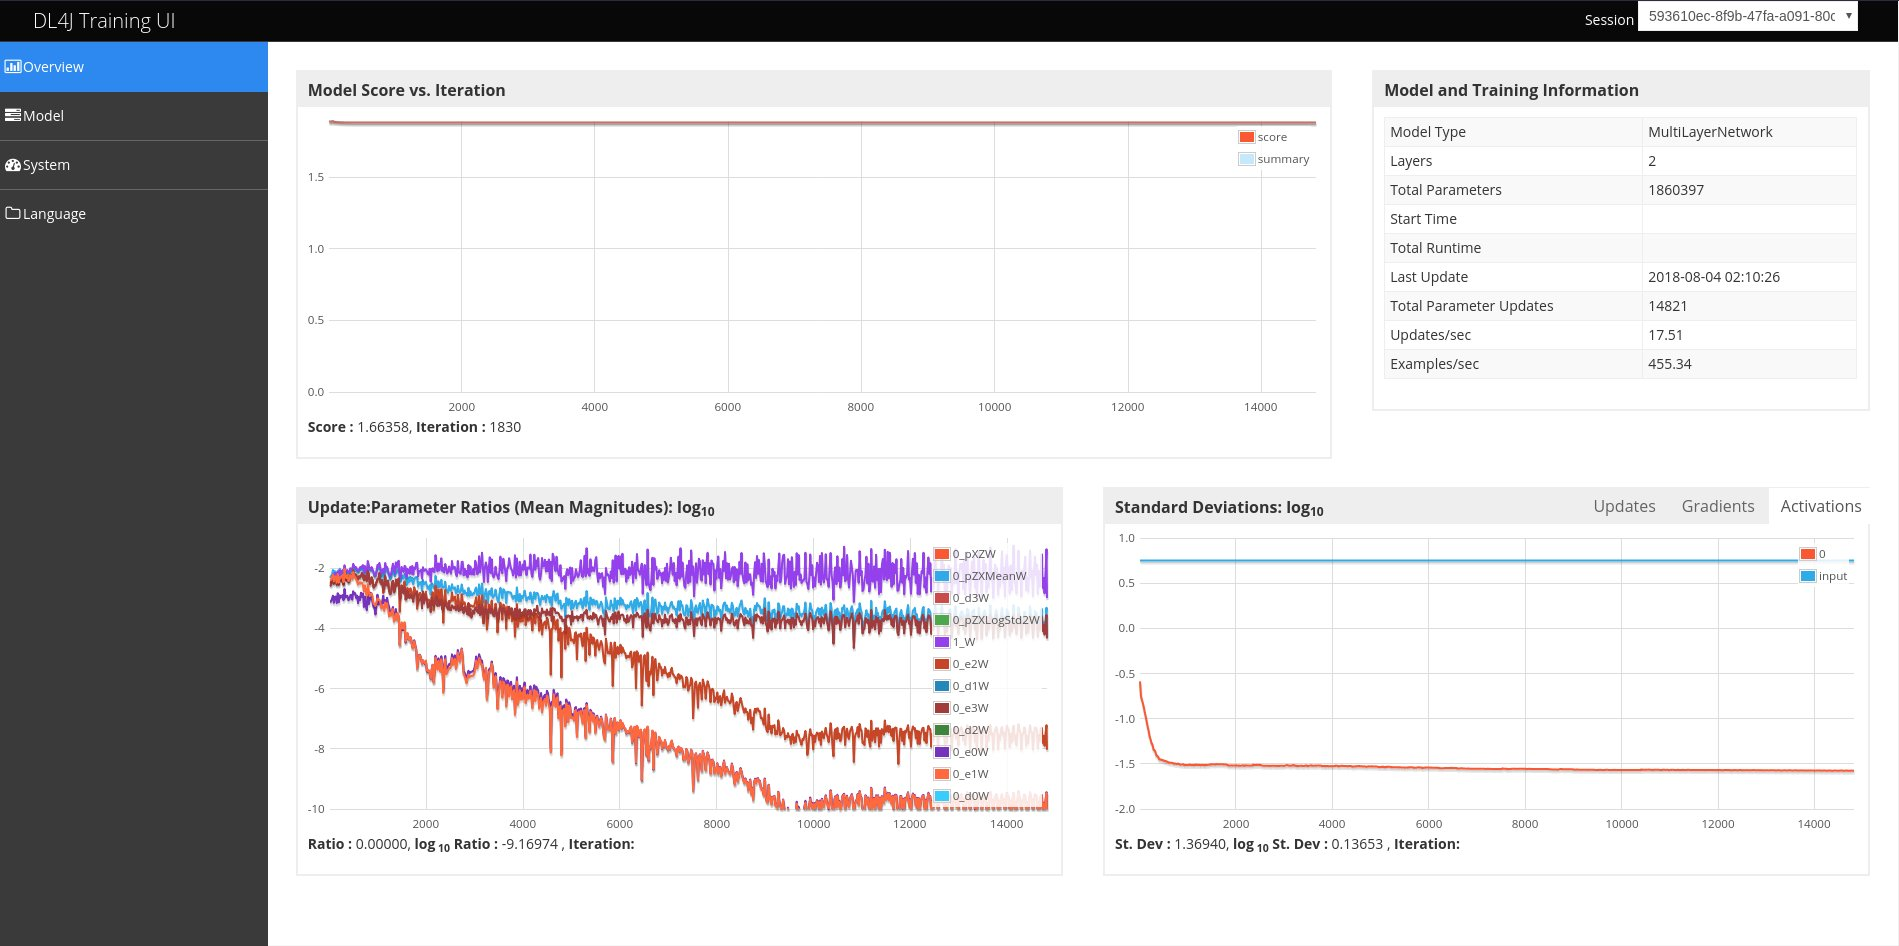
\includegraphics[width=12cm]{./failed_qna.jpg}
\caption{\label{fig:org25df6f9}
上手く行かなかった例}
\end{figure}

\begin{figure}[htbp]
\centering
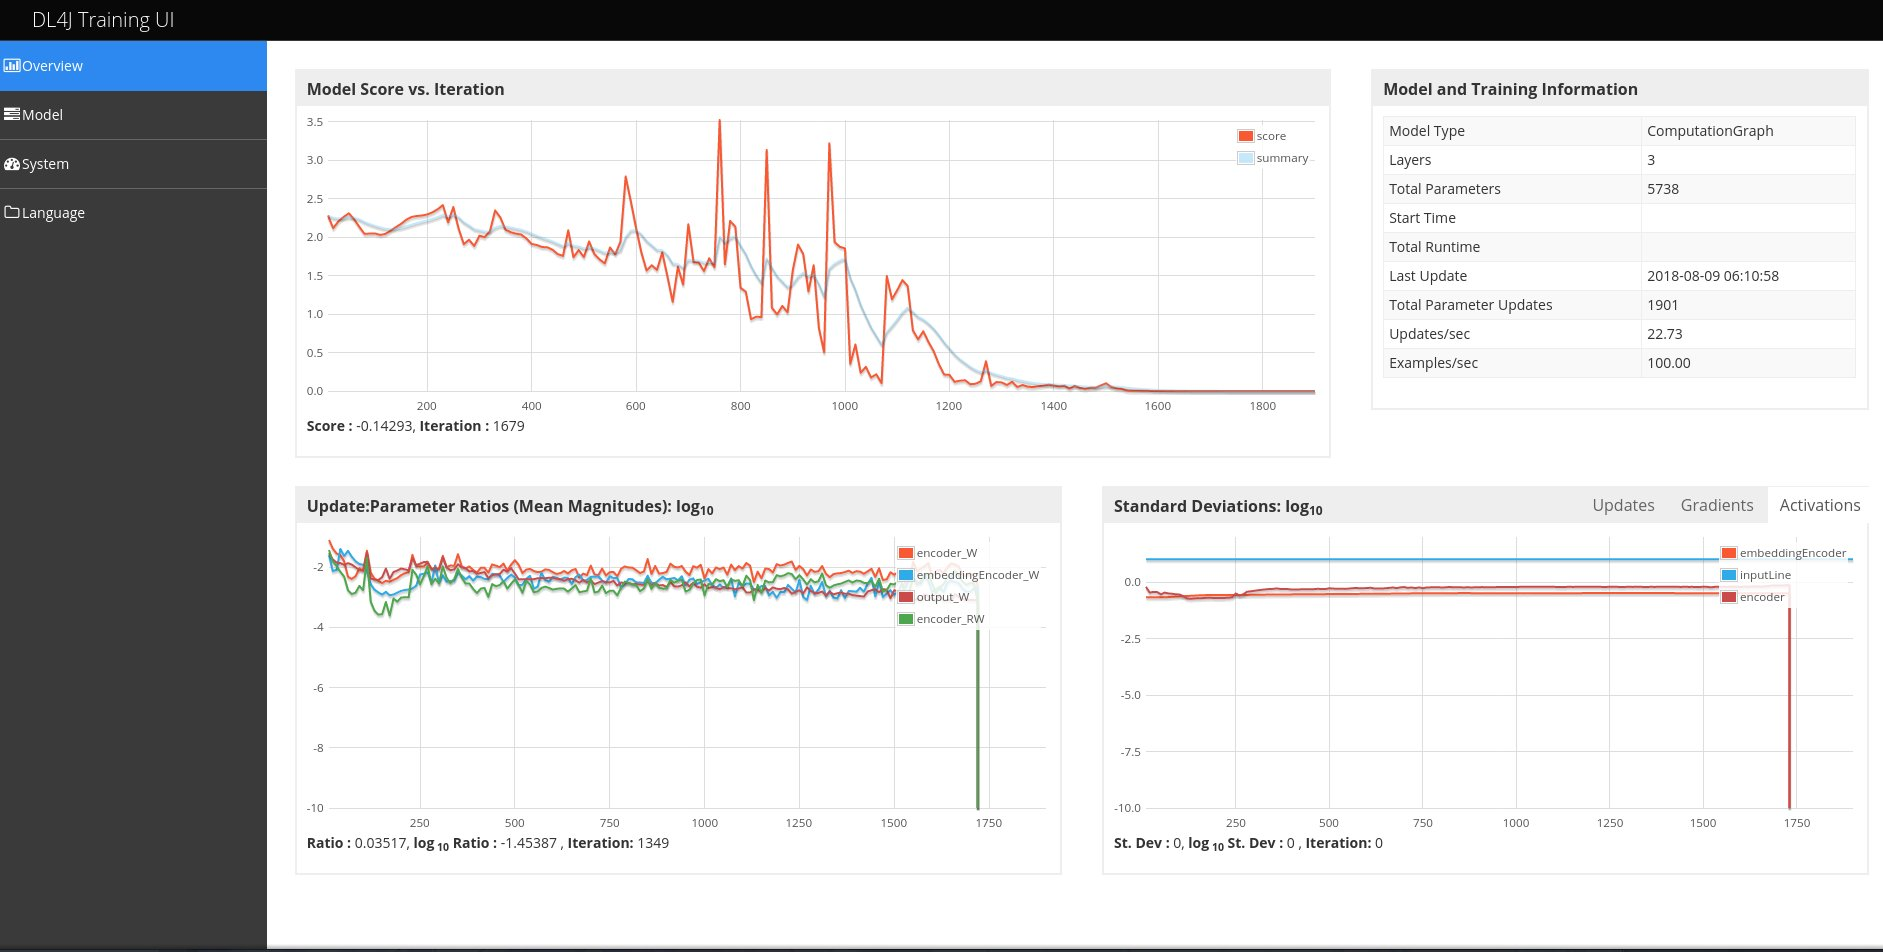
\includegraphics[width=12cm]{./success_qna.jpg}
\caption{\label{fig:orge69aa1b}
Seq2Labelを使った例}
\end{figure}

\begin{figure}[htbp]
\centering
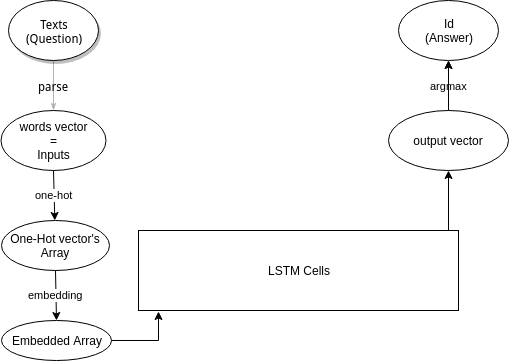
\includegraphics[width=12cm]{./Diagram.png}
\caption{\label{fig:org3d3094e}
Seq2Labelの概要}
\end{figure}

 しかしいくつかの実験を行った結果、このモデルの欠陥をいくつか発見した。また日本語特有の問題もあるが、これについては \ref{sec:orgcb39560} で説明する。\\
\begin{itemize}
\item モデルが収束しすぎる。\\
 余りにも質問文の内容が乖離しすぎていると深層学習する必要がなくなってしまう。また誤差逆伝搬法で問題が起きる(NaN 値を発生してしまう。)\\
\item 単語数が増えると空間計算量が増える。\\
 空間計算量を減らしすぎると今度はモデルが上手くフィットしない。\\
\end{itemize}

\section{データセットの作成}
\label{sec:orgcb39560}
 日本語のデータセットを収集する必要があったが良質と思われる \footnote{例えば後述する CopyNet や HRED などではQ\&Aではなく、 \textbf{意味の通る} 長い会話データが必要となる。\\} データセットが見つからず、実際にデータセットを作成することにした。また時間があればこのデータセットと他のデータセットを比較してみようと考えている。\footnote{しかしデータの前処理によってもデータが大きく変化してしまうので実験は難しいと考えられる。\\}\\
 作成しているデータセットはMITライセンスで公開する \footnote{\url{https://github.com/MokkeMeguru/japanese-corpus}\\}ことで他の研究者からの意見を聞きたいと考えている。\\
 また、最終的には Seq2Seq で使われる既存のデータセットの中で最小となっていた 3k を目指している。\\
 文脈不明・理解不能な会話文が一切ないため、低品質なデータセットに比べてもそれなりの成果が得られると予想している。\\
\section{Seq2Seq attention の理解}
\label{sec:orgddd7f93}
 deeplearning4j では Seq2Seq が実装できず、 Seq2Seq attention \footnote{\url{https://qiita.com/kenchin110100/items/eb70d69d1d65fb451b67}\\} が実装でき、公式のサンプルがその実装例を紹介している。そのため、このソースコードの理解を以てこのモデルを理解したことになると考えている。\footnote{\url{https://github.com/MokkeMeguru/seq2seq-memo}\\}\\

\begin{figure}[htbp]
\centering
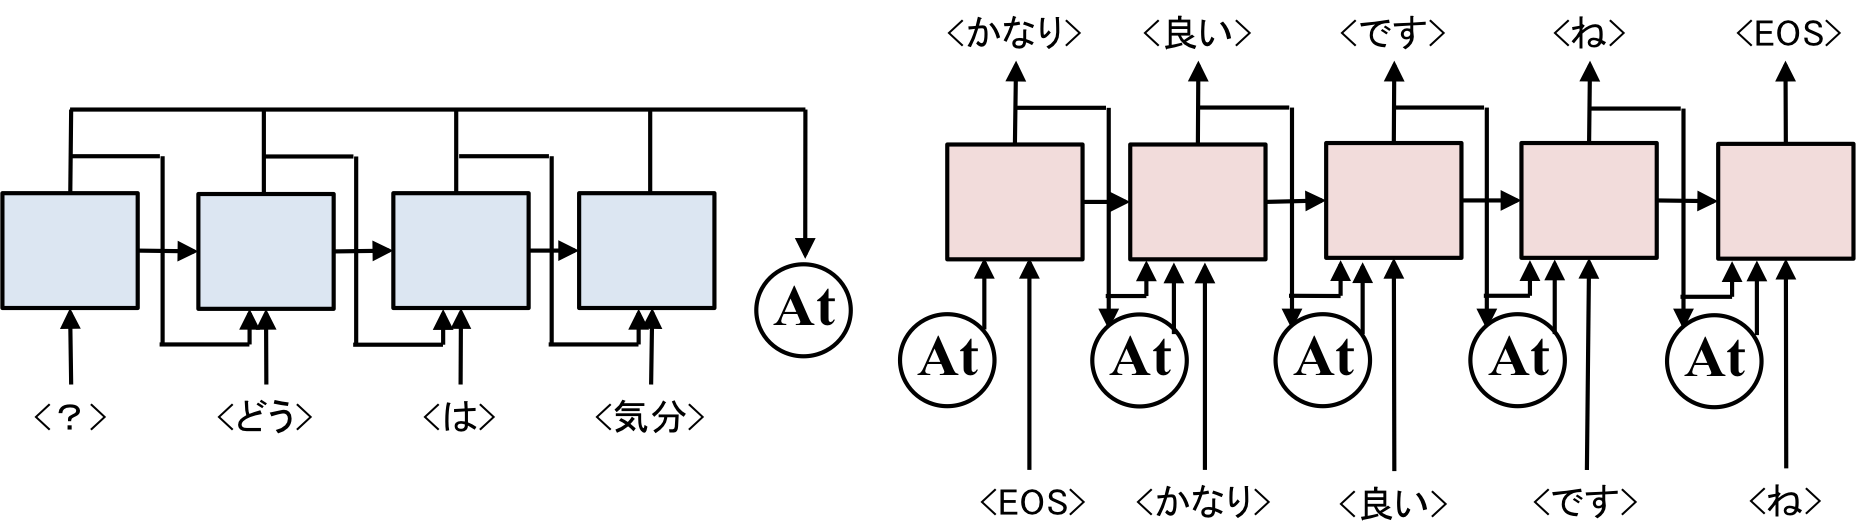
\includegraphics[width=12cm]{./seq2seq_att.png}
\caption{\label{fig:org483d507}
Seq2Seq Attention のモデル図}
\end{figure}

\section{word2vec の理解と実装}
\label{sec:org74992ff}
 こちらに関しては deeplearning4j が完全にサポートしており、文字通り一行でモデルを作ることが出来る。これを用いて、qna システム内 の Encoder 部分に適用した際の適合率について比較を行いたいと考えている。(seq2seqではいくつかの特殊なTokenが存在するため用いることが出来ない。)\footnote{\url{https://github.com/MokkeMeguru/word2vec\_memo}\\}\\

\section{doc2vec の利用方針}
\label{sec:org3dbdd3c}
 IBM のチャットボット Watson では質問文を細かくカテゴライズするという手法を取っている。\footnote{\url{https://www.ibm.com/blogs/solutions/jp-ja/watson-machinelearning-2/} この実装と本研究の共通点は、どちらも「手で」データを選別(生成)しているということである。\\}\\
 データの面でのカテゴライズはデータセット生成の時点で済ませてあるものとしてみなすことが出来るため、問題となるのは入力後のデータ処理についてである。この、入力された後のデータ分類を doc2vec を用いて行いたいと考えている。この実装はデータセットが目標数に達成したところで、 deeplearning4j のドキュメントを参考に実装していく予定である。\\
\section{文体変換について}
\label{sec:org6a6190c}
 文体変換についてはいくつかの手法を検討している。\\
 例えば日本語で研究が行われた先行例として、転移学習を用いたもの \cite{stkn_tohoku} がある。\\
 本研究ではこれに加えて、転移学習についていくつかの手法を提案する他、VAE を用いたパターン、Zero-shot 変換を用いたパターン、Seq2Seq attention (応答->応答) 、などを実験する予定である。\\
\section{全体的なシステムの想定図}
\label{sec:org2aa07d0}
別紙を参照\\

\printbibliography[title=参考文献]
\end{document}
